 \section{Balanced Scorecard} 

{\Large Las 4 perspectivas dentro del Balanced Scorecard.-}\\
Una metodología muy utilizada por las organizaciones en la actualidad para lograr la alineación de los objetivos de la empresa con los de cada uno de los miembros del equipo es el Balanced Scorecard el cual tiene como principal fin fungir como una herramienta de medición y de gestión que permite direccionar los esfuerzos del talento humano para traducir la estrategia en ejecución.


El BSC es una herramienta de gestión que convierte la visión de la compañía en acciones concretas mediante un conjunto de indicadores divididos en 4 categorías del negocio, las cuales son las siguientes:
 
\begin{itemize}
		\item Financiera
		\item Enfoque en el cliente
		\item Procesos internos
		\item Aprendizaje y crecimiento
\end{itemize}

\begin{center}
	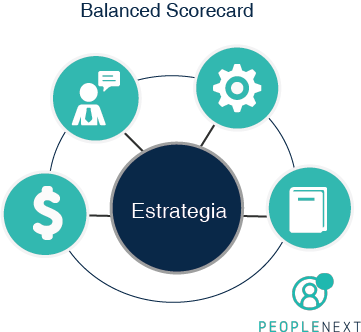
\includegraphics[width=10cm]{./Imagenes/imagen1} 
\end{center}
Se considera que en estos 4 rubros se engloban todos los procesos que la empresa requiere para un correcto funcionamiento y deben de tomarse en cuenta para definir los indicadores clave de la compañía. Es importante el equilibrio entre estas categorías ya que es lo que otorga el balance entre los procesos internos que tienen que ver con colaboradores, innovación, capacitación, etc así como los externos que van relacionados a los accionistas y clientes.\\
\pagebreak

\subsection{Perspectiva financiera}

Esta categoría dentro de los objetivos del Balanced Scorecard tiene como objetivo responder a las expectativas de los accionistas, su principal enfoque es crear valor para ellos mediante indicadores de rendimiento que reflejen el comportamiento operativo, crecimiento y sustentabilidad de la empresa.\\
-
La perspectiva financiera del BSC es el vínculo final de los objetivos de cada unidad de negocio con la estrategia organizacional, es decir la meta final que se persigue en la empresa, generar utilidad. Ésta es muy importante para analizar el desempeño de la empresa como generadora de ingresos.\\
-
Por lo general este rubro incluye objetivos de índole estratégico como el incremento de los ingresos, el aumento en las utilidades, la mejora en las operaciones y utilización de recursos y capital.\\

Algunos indicadores comunes en esta perspectiva son:
\begin{itemize}
	\item Ingresos
	\item Utilidad neta
	\item Valor económico agregado
	\item Margen operativo
	\item Margen de contribución
	\item Retorno de la inversión
	\item Flujo de caja
	\item Precio de la acción
\end{itemize}
La importancia de esta perspectiva radica en dar a conocer a los accionistas información precisa y actualizada sobre el desempeño financiero de la empresa y conocer si el negocio está siendo rentable de acuerdo a las metas estratégicas establecidas.\\

\begin{center}
	
\includegraphics[width=12cm]{./Imagenes/imagen2} 
\end{center}

\pagebreak

\subsection{Perspectiva de enfoque en el cliente}

En este apartado del cuadro de mando es importante centrarse en lo que la empresa requiere llevar a cabo para garantizar la retención del cliente y la adquisición de clientes futuros para brindar rentabilidad a la organización. En esta categoría se brinda información de la percepción del cliente y con base a ello se definen indicadores que ayudarán a responder a las expectativas de los clientes. De esto depende en gran parte la generación de ingresos que se verán reflejados en la perspectiva financiera.\\

Algunos indicadores comunes en esta perspectiva son:
\begin{itemize}
	\item Nivel de satisfacción del cliente
	\item Índice de recompra
	\item Participación de mercado
	\item Pedidos devueltos
	\item Percepción de valor de marca.
	\item Cantidad de quejas.
\end{itemize}

\begin{center}
	
\includegraphics[width=12cm]{./Imagenes/imagen3} 
\end{center}
Es importante dar el valor a esta categoría como parte esencial de la estrategia organizacional para buscar un enfoque en el cliente que le permitirá a la compañía alcanzar de manera satisfactoria sus metas y destacarse frente a la competencia.\\
\pagebreak

\subsection{Perspectiva de procesos internos}

En esta categoría se deben identificar los objetivos estratégicos que están relacionados directamente con los procesos clave de la organización de los cuales depende cubrir las expectativas tanto de accionistas como de los clientes. \\
Por lo general el diseño de los indicadores de esta perspectiva se realiza cuando ya se han definido los mismos para la perspectiva financiera y la de enfoque en el cliente, ya que ésta busca la alineación de las actividades de los colaboradores con los procesos clave de la empresa para con esto establecer los objetivos estratégicos. \\
De esta manera se pueden revisar y mejorar los procedimientos internos que conforman la cadena de valor la cual tiene como inicio el proceso de innovación siguiendo con los operativos y terminando con el servicio post-venta que brindan el valor agregado a los clientes.\\
En particular en este rubro del Cuadro de Mando es importante que esté adecuado y diseñado según las operaciones de la empresa y que se desarrolle tomando como punto de partida la cadena de valor y/o el modelo de negocio sobre el cual se basan las actividades de la empresa.\\

Algunos indicadores comunes en esta perspectiva son:\\

\textbf {Procesos de innovación}
\begin{itemize}
	\item Porcentaje de nuevos productos y/o servicios.
	\item Costos de desarrollo de nuevos productos y/o servicios.
	\item Porcentaje de ventas de nuevos productos y/o servicios.
\end{itemize}

\textbf {Procesos operativos}
\begin{itemize}
	\item Porcentaje de mermas
	\item Margen de productos defectuosos
	\item Devoluciones por producto defectuoso
	\item Tiempos de fabricación
	\item Aprovechamiento de activos
\end{itemize}

\textbf {Procesos de post-venta}
\begin{itemize}
	\item Tiempo de respuesta al cliente
	\item Costo de las reparaciones
	\item Cumplimiento de garantías
\end{itemize}
\pagebreak

\subsection{Perspectiva de aprendizaje y crecimiento}

Es en este rubro en que la empresa debe poner especial atención para obtener resultados a largo plazo, dentro de éste se pueden identificar tres áreas principales:\\

Algunos indicadores comunes en esta perspectiva son:\\

\textbf {Capital Humano}
\begin{itemize}
	\item Se refiere al conocimiento que tiene el equipo de trabajo así como su capacidad para aprender y adaptarse a los nuevos retos en el ámbito laboral.
\end{itemize}

\textbf {Sistemas e infraestructura}
\begin{itemize}
	\item En este apartado se incluye el apoyo tecnológico, la información y los recursos que la empresa brinda a su talento humano para llevar a cabo sus actividades de manera más efectiva. 
\end{itemize}

\textbf {Clima organizacional}
\begin{itemize}
	\item Este factor es de gran relevancia ya que su medición indica cómo se sienten tus colaboradores trabajando para la empresa, si se identifican con sus valores y las percepciones que tienen acerca de las oportunidades de cambio que pueden ayudar a mejorar la empresa como lugar de trabajo. Esto generalmente tiene repercusiones a nivel productividad, rotación de personal etc. 
\end{itemize}
Como se puede observar en las perspectivas anteriores (financiera, enfoque a clientes y procesos internos) se busca la excelencia para alcanzar los objetivos de la organización mediante procesos clave; sin embargo, en la perspectiva de aprendizaje y desarrollo el punto principal está en el talento humano el cual funge como el medio para alcanzar ese nivel de excelencia y lograr los objetivos estratégicos, son quienes lo llevan a cabo. \\
\pagebreak
